\documentclass[10pt,conference]{IEEEtran}
\IEEEoverridecommandlockouts
% PAPER v2 -- DRAFT. Every number, table and figure is PROVISIONAL, pending the owner's human labels.
% Paper v1 is a separate, frozen document and is not changed by this draft.
\usepackage{cite}
\usepackage{amsmath,amssymb}
\usepackage{booktabs}
\usepackage{graphicx}
\usepackage[table]{xcolor}
\usepackage{url}
\usepackage{array}
\usepackage{tikz}
\usetikzlibrary{positioning,arrows.meta,calc}
\usepackage[hidelinks]{hyperref}
\usepackage{draftwatermark}
\SetWatermarkText{PROVISIONAL}
\SetWatermarkScale{0.9}
\SetWatermarkColor[gray]{0.92}
\definecolor{oiVerm}{HTML}{D55E00}
\newcommand{\prov}{\textcolor{oiVerm}{\textbf{[provisional, pending human labels]}}}
\newcommand{\sys}{Odin}
\newcommand{\nTrainSyn}{836}
\newcommand{\nStrictDtwo}{42}
\newcommand{\nExtDtwo}{67}
\newcommand{\nDone}{39}
\newcommand{\layerFive}{mean16-24}
\newcommand{\layerFifteen}{L24}
\newcommand{\prefixTokens}{925}
\newcommand{\prefixMsFive}{170}
\newcommand{\loadSFive}{1.6}
\newcommand{\dOneLlmMed}{10.7}
\newcommand{\dOneJevMed}{28}
\newcommand{\dTwoRouterMed}{906}
\newcommand{\dTwoJevMed}{24}
\newcommand{\dTwoClaudeMed}{10.9}
\newcommand{\dOneUsd}{2.785}
\newcommand{\dTwoClaudeUsd}{2.37}

\begin{document}
\title{A Local, Calibrated Decider for Closed Decisions in an Agentic Orchestrator\\
\large DRAFT -- all results provisional, pending human labels}
\author{\IEEEauthorblockN{Mostafa A. M. Sayed Adawy}\IEEEauthorblockA{[Affiliation to be confirmed by the author]\\ {mostafa\_adawy@ymail.com}}}
\maketitle
\begin{abstract}
\sys{} is an agentic orchestrator in which a large language model (LLM) currently makes every routing decision, including \emph{closed} decisions with a fixed list of answers: whether a request needs one specialist or a team, which specialist owns it, whether it only reads or changes state, whether a project needs a QA gate, and whether a team member is technical. Each such call costs seconds and plan usage. We add \emph{Jev mode}: a local decider that runs on the owner's Apple M4 laptop. A frozen Qwen2.5 model reads a cached standing context once; small per-decision heads read one hidden state and answer in tens of milliseconds, with a calibrated confidence. Below a threshold set so that the decider is never less accurate than the LLM on validation data, the case goes back to the LLM. Truth for validation and testing comes only from what the logs show was done and accepted, or from the owner's own words, never from the LLM or the router being compared. On the current held-out set the decider matches the production path on mode (\nDone{} cases) and on read/change (\nStrictDtwo{} cases) at roughly $1/40$ to $1/380$ of the decision time; no accuracy difference is statistically significant. End to end, the agents' own work and its run-to-run variance dominate: the decider removes about 7\,s of LLM time before the agent starts, but with 6--9 runs per mode no end-to-end difference can yet be measured in either direction. \prov{}
\end{abstract}

\section{Introduction}
\sys{} routes owner requests through an LLM at several points. Many of these points are closed decisions with two to seven fixed options. Using a general LLM for them has three costs: latency (a median of \dOneLlmMed{}\,s for the mode decision on our test set), usage (\$\dOneUsd{} of reported plan usage per pass over the mode test set, not charged), and dependence on the network. This draft describes a local alternative and how it was measured. Its contributions are:
\begin{itemize}
\item a frozen-encoder decider with a prepared standing-context cache, per-decision heads, temperature scaling, and an LLM fallback threshold that is never set below the LLM's own validation accuracy (Section~\ref{sec:method});
\item a ground-truth protocol that excludes every LLM and router decision output, with rules over the logs and an owner review sample (Section~\ref{sec:truth});
\item a paired evaluation with confidence intervals and exact McNemar tests, an explicit \emph{non-inferior} acceptance rule, and a shadow mode that gives the decider no live authority until human labels exist (Sections~\ref{sec:protocol}--\ref{sec:results}).
\end{itemize}

\section{Why a cloud decider was rejected}\label{sec:rejected}
A hosted classification service was evaluated first and rejected by the owner for five reasons: (1) it is paid; (2) it is cloud-only, so decision data would leave the laptop and the decider would need internet access, which conflicts with \sys{}'s offline Anchor path; (3) the network round-trip from the owner's location removes most of its speed advantage; (4) its API is stateless, so the standing context has to be resent with every call; (5) it decides only from what it is given, whereas \sys{}'s LLM can search and gather context before deciding. The local design below keeps all data on the machine, needs no network, and prepares the standing context once.

\section{Method}\label{sec:method}
\subsection{Decision points}
Jev covers five closed decisions already present in \sys{}: \emph{mode} (direct or orchestrate, in the request classifier), \emph{specialist} and \emph{read/change} (in the dispatcher), \emph{QA gate} (the QA recommendation when a project is created), and \emph{agent nature} (technical or operational, when an agent is proposed). Each call site asks the decider first; a \texttt{None} answer means ``use the existing LLM path unchanged''. Requests that contain an owner exclusion (``do not'', ``only'', ``read-only'', \ldots) always go to the LLM.
\subsection{Encoder and standing context}
A Qwen2.5 instruction model~\cite{qwen25} runs frozen in MLX~\cite{mlx} on the M4 GPU. The standing context (\sys{}'s specialists, rules, real agents and projects; \prefixTokens{} tokens) is run once and kept as a key/value cache~\cite{pope2023}; it takes \prefixMsFive{}\,ms to prepare with the 0.5B model. Each decision only processes its short suffix (decision definition and the input). We take the last token's hidden state.
\subsection{Layer choice}
Intermediate layers of a transformer often separate task-relevant information better than the last layer~\cite{alain2017,belrose2023}. We compare the states after layers 12, 16, 20, 24 and 28, the mean of layers 16--24, and the final normed state (Table~\ref{tab:layers}); one forward pass yields all of them. The kept layer is \layerFive{} for 0.5B and \layerFifteen{} for 1.5B, chosen on the synthetic validation split. \prov{} After the owner's labels, the choice is re-made on the real validation set.
\subsection{Heads, calibration and fallback}
Each decision has a two-layer MLP head (256 hidden units) trained with class weights on generated data. Probabilities are calibrated with temperature scaling~\cite{guo2017} (grid 0.05--100, fitted by negative log-likelihood). The fallback threshold $\tau$ is the lowest confidence at which the decider's accuracy on the kept validation cases is at least the LLM's validation accuracy; below $\tau$ the case returns to the LLM, a selective-prediction scheme~\cite{geifman2017}. A head with fewer than 5 independent validation labels is \emph{off}; a class with fewer than 5 independent cases is \emph{off} (that answer always goes to the LLM); a class with fewer than 20 training examples is grouped and always goes to the LLM.
\subsection{Overhead on the request path}
Two sources of overhead added by the decider itself were found in the timing analysis (Section~\ref{sec:results}) and removed. (i) In shadow mode the decider ran \emph{on} the request path, about 40\,ms per chat turn whose answer is never used; it now runs on a background worker that writes the same log record, and the request path pays 0.3\,ms (measured on the M4 with the real model). (ii) The first decision after start paid about 1.5\,s to load the model and build the context cache; both are now pre-warmed in the background when the brain starts and when Jev is switched on, and the first real decision takes 72\,ms. Regression tests cover both (``shadow adds no latency and ``pre-warm). \prov{}
\subsection{Authority}
The mode switch (Normal / Jev) is in the desktop app. Until the owner's labels arrive, Jev runs in \emph{shadow}: the decider runs and is logged, but the LLM decides every case. Only the post-label re-run may grant live authority.
\begin{figure}[t]\centering
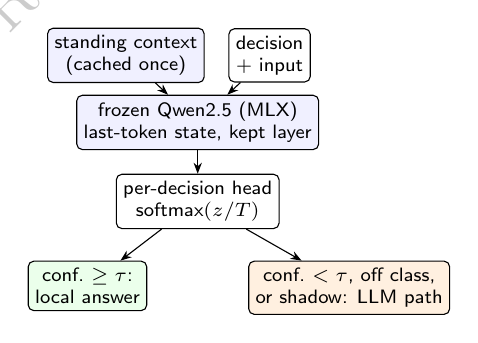
\begin{tikzpicture}[font=\sffamily\scriptsize,node distance=3mm,
 b/.style={draw,rounded corners=2pt,align=center,inner sep=2.5pt,fill=white},
 a/.style={-{Stealth[length=1.4mm]}}]
\node[b,fill=blue!6] (ctx) {standing context\\(cached once)};
\node[b,right=of ctx] (in) {decision\\+ input};
\node[b,below=5mm of $(ctx)!0.5!(in)$,fill=blue!6] (enc) {frozen Qwen2.5 (MLX)\\last-token state, kept layer};
\node[b,below=of enc] (head) {per-decision head\\softmax$(z/T)$};
\node[b,below left=4mm and -4mm of head,fill=green!8] (loc) {conf.\ $\ge\tau$:\\local answer};
\node[b,below right=4mm and -4mm of head,fill=orange!12] (llm) {conf.\ $<\tau$, off class,\\or shadow: LLM path};
\draw[a] (ctx) -- (enc); \draw[a] (in) -- (enc); \draw[a] (enc) -- (head); \draw[a] (head) -- (loc); \draw[a] (head) -- (llm);
\end{tikzpicture}
\caption{The Jev decider. Low confidence, disabled classes and shadow mode all return the case to the existing LLM path.}
\label{fig:arch}\end{figure}

\section{Training data and ground truth}\label{sec:truth}
\subsection{Training data}
Training examples were generated with an LLM (plan login, no extra cost) from \sys{}'s real context: project names, agent roster, and the exact decision definitions. Real test inputs were never shown to the generator; any generated example too close to a real input (token Jaccard $>0.70$ or character similarity $>0.80$) was removed. For agent nature, 20 descriptions were generated for each of 39 agent families seen in the real roster. After leakage removal, 2{,}179 examples remain: 1{,}864 for training and 315 (15\%) as a synthetic validation split. These labels come from an LLM, so they are used only for training and the synthetic split, never as truth.
\subsection{Independent truth}
A validation or test label may come only from evidence that does not depend on the LLM or router being compared:
\begin{itemize}
\item \emph{owner correction}: the owner's next message states what he wanted (``I'm not asking about deployment, only \ldots'');
\item \emph{accepted outcome}: the logged reply shows what was actually done, and the owner's next message does not complain or correct it; for mode, only an accepted single direct reply counts, because an accepted team run does not prove a team was needed;
\item \emph{owner's words}: the owner's own brief or message states it (``no QA agent''; ``build \ldots, QA, then deploy'').
\end{itemize}
The rules are regular expressions over the logs, and every label keeps its evidence. The labelling script reads no router or LLM decision field; on read/change its labels disagree with the router on 9 of 55 cases. Strict truth currently covers mode (49 direct, 2 orchestrate), read/change (43 read, 12 change) and QA gate (8 ``no''). Specialist and agent nature have no strict log truth: the logs show who \emph{executed} a request (mostly the CTO agent), not who should \emph{own} it.
\subsection{Extended read/change truth}
To grow the read/change set, a second rule set was written for this decision only: a read-only reply that the owner did not dispute as to action type, a change the owner did not dispute, or a change approval the owner granted. It adds 37 cases. Inspection showed these rules make errors (for example, a request to build an app labelled ``read'' because the reply only planned), so extended results are reported separately and never as the headline. All 176 unique owner messages in the logs have been examined; the logs cannot reach 100 strict read/change cases.
\subsection{Owner review}
A stratified sample of 90 items (specialist 29, read/change 18, mode 15, QA 14, agent nature 14) waits for the owner's review on a private page. Only answered items become truth. \prov{}

\section{Evaluation protocol}\label{sec:protocol}
Real inputs are split per kind into validation (30\%) and held-out test (70\%) with a fixed seed. The test split is never used for training or tuning. Each comparison runs every test case three times through \sys{}'s own code paths. The production path is Claude for mode and QA gate, and the local semantic router for read/change; for read/change we add a Claude classifier with the same standing context and definition.
For each method a case is correct when it is correct in the majority of its repetitions. We report accuracy with 95\% Wilson intervals~\cite{wilson1927} and test paired differences with the exact McNemar test~\cite{mcnemar1947}. Calibration is the expected calibration error (ECE, 10 bins~\cite{naeini2015}) of the decider before and after temperature scaling. We also report decision time, end-to-end time in real scenarios, reported plan usage (not charged), and fallback rate.
\textbf{Acceptance rule.} \emph{Best}: significantly more accurate ($p<0.05$) and faster. \emph{Non-inferior}: the same accuracy and faster, or higher but not significant; the LLM still handles every low-confidence case. \emph{Inconclusive}: lower but not significant. \emph{Failure}: significantly less accurate, or the same or worse accuracy with no speed gain.

\section{Results (provisional)}\label{sec:results}
\textbf{All numbers in this section are provisional, pending the owner's human labels.} They will be regenerated, in a fixed order (layer choice on the real validation set, temperature scaling, thresholds, then the head-to-head), once the labels exist.
\begin{table}[t]\centering\scriptsize
\caption{Layer comparison on the synthetic held-out validation split (15\% of the generated data). Mean = mean accuracy over the five decisions; $\star$ = kept. \textbf{PROVISIONAL -- pending human labels}.}
\label{tab:layers}\setlength{\tabcolsep}{3.5pt}
\begin{tabular}{lrrr rrr}\toprule
 & \multicolumn{3}{c}{Qwen2.5-0.5B (24 layers)} & \multicolumn{3}{c}{Qwen2.5-1.5B (28 layers)}\\
\cmidrule(lr){2-4}\cmidrule(lr){5-7}
Layer & Mean & R/C acc & R/C ECE & Mean & R/C acc & R/C ECE\\\midrule
12 & 91.6 & 92.9 & 0.052 & 91.2 & 93.6 & 0.063 \\
16 & 91.6 & 96.2 & 0.042 & 91.1 & 95.5 & 0.044 \\
20 & 91.6 & 94.9 & 0.043 & 91.7 & 96.2 & 0.043 \\
24 & 91.9 & 96.8 & 0.039 & 93.7 $\star$ & 97.4 & 0.030 \\
28 & n/a & n/a & n/a & 93.6 & 96.8 & 0.034 \\
mean 16--24 & 93.0 $\star$ & 95.5 & 0.045 & 93.4 & 95.5 & 0.041 \\
final (normed) & 92.2 & 96.8 & 0.037 & 93.2 & 96.8 & 0.031 \\
\bottomrule\end{tabular}\end{table}

\begin{table}[t]\centering\scriptsize
\caption{Per-class recall (\%) at the kept layer, synthetic held-out validation split. \textbf{PROVISIONAL -- pending human labels}.}
\label{tab:recall}\setlength{\tabcolsep}{3pt}
\begin{tabular}{l l p{4.6cm}}\toprule Decision & Model & Recall per class\\\midrule
Mode (direct / orchestrate) & 0.5B & direct 99, orchestrate 80 \\
Mode (direct / orchestrate) & 1.5B & direct 99, orchestrate 73 \\
Specialist & 0.5B & Frontend 71, Backend 75, DevOps \& Cloud 71, Security \& Compliance 80, QA \& Testing 91, Database 85, CTO Brain 81 \\
Specialist & 1.5B & Frontend 81, Backend 75, DevOps \& Cloud 89, Security \& Compliance 80, QA \& Testing 100, Database 85, CTO Brain 62 \\
Read / change & 0.5B & read 96, change 94 \\
Read / change & 1.5B & read 100, change 92 \\
QA gate & 0.5B & no 100, yes 91 \\
QA gate & 1.5B & no 95, yes 91 \\
Agent nature & 0.5B & technical 98, operational 99 \\
Agent nature & 1.5B & technical 97, operational 100 \\
\bottomrule\end{tabular}\end{table}

\subsection{Layers}
Table~\ref{tab:layers} compares layers on the synthetic validation split. Differences between layers are within about two points of mean accuracy; the mean of layers 16--24 is best for 0.5B and layer 24 for 1.5B. Specialist is the hardest decision (Table~\ref{tab:recall}).
\begin{table*}[t]\centering\scriptsize
\caption{Head-to-head on the held-out test split (strict independent truth), 3 repetitions. A case counts as correct when it is correct in the majority of its repetitions; 95\% Wilson intervals; exact McNemar test on the discordant cases ($b$ = only Jev right, $c$ = only the production LLM path right). Mode and QA gate: the production path is Claude; read/change: the production path is the local semantic router. \textbf{PROVISIONAL -- pending human labels}.}
\label{tab:h2h}
\begin{tabular}{l l r l l r r r}\toprule
Decision & Jev model & $n$ & Production path acc.\ \% [95\% CI] & Jev acc.\ \% [95\% CI] & $b/c$ & McNemar $p$ & Fallback \%\\\midrule
Mode (direct / orchestrate) & 0.5B & 39 & 100.0 [91.0, 100.0] & 100.0 [91.0, 100.0] & 0/0 & 1.000 & 5 \\
Read / change & 0.5B & 42 & 83.3 [69.4, 91.7] & 83.3 [69.4, 91.7] & 1/1 & 1.000 & 12 \\
QA gate & 0.5B & 7 & 71.4 [35.9, 91.8] & 71.4 [35.9, 91.8] & 0/0 & 1.000 & 100 \\
Mode (direct / orchestrate) & 1.5B & 39 & 100.0 [91.0, 100.0] & 100.0 [91.0, 100.0] & 0/0 & 1.000 & 5 \\
Read / change & 1.5B & 42 & 83.3 [69.4, 91.7] & 88.1 [75.0, 94.8] & 3/1 & 0.625 & 0 \\
QA gate & 1.5B & 7 & 71.4 [35.9, 91.8] & 71.4 [35.9, 91.8] & 0/0 & 1.000 & 100 \\
\bottomrule\end{tabular}\end{table*}

\begin{table*}[t]\centering\scriptsize
\caption{Read/change: Jev against a Claude classifier (plan login, same standing context and definition) and the production router. Strict = log-outcome truth with owner acceptance; extended = additional log rules for this decision only, lower confidence (Section~\ref{sec:truth}). McNemar against Claude. \textbf{PROVISIONAL -- pending human labels}.}
\label{tab:claude}
\begin{tabular}{l l r r l l r r}\toprule
Truth set & Jev & $n$ & Router \% & Claude \% [95\% CI] & Jev \% [95\% CI] & $b/c$ & McNemar $p$\\\midrule
strict & 0.5B & 42 & 83.3 & 73.8 [58.9, 84.7] & 83.3 [69.4, 91.7] & 5/1 & 0.219 \\
strict & 1.5B & 42 & 83.3 & 73.8 [58.9, 84.7] & 88.1 [75.0, 94.8] & 8/2 & 0.109 \\
strict + extended & 0.5B & 67 & 74.6 & 74.6 [63.1, 83.5] & 80.6 [69.6, 88.3] & 7/3 & 0.344 \\
strict + extended & 1.5B & 67 & 74.6 & 74.6 [63.1, 83.5] & 83.6 [72.9, 90.6] & 11/5 & 0.210 \\
\bottomrule\end{tabular}\end{table*}

\subsection{Held-out head-to-head}
On mode, the decider and the production path are both correct on all \nDone{} test cases; the set contains only one ``orchestrate'' case, and that class is off, so this result shows only that the decider answers ``direct'' cases correctly. On read/change (\nStrictDtwo{} cases), the 0.5B decider has the same accuracy as the router and the 1.5B decider is higher, but the difference is not significant (Table~\ref{tab:h2h}). Against the Claude classifier both deciders are higher, again without significance (Table~\ref{tab:claude}). Under the acceptance rule every measured result is \emph{non-inferior}; none is \emph{best}. The QA gate, specialist and agent-nature heads are off.
\begin{figure}[t]\centering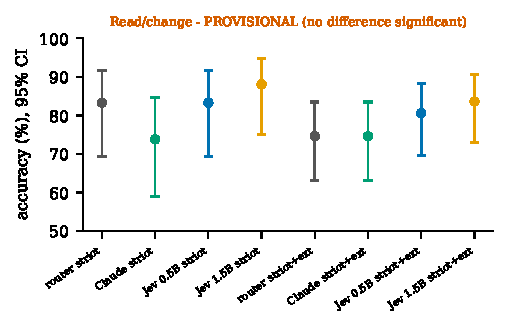
\includegraphics[width=\columnwidth]{figs/rc_acc.pdf}
\caption{Read/change accuracy with 95\% Wilson intervals. The intervals overlap; no difference is significant. \prov{}}\label{fig:rc}\end{figure}
\begin{figure}[t]\centering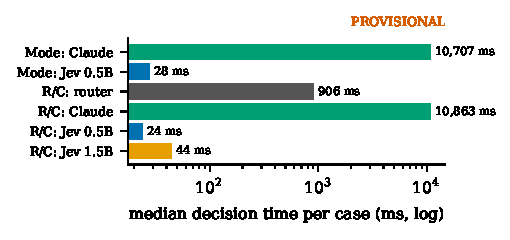
\includegraphics[width=\columnwidth]{figs/latency.pdf}
\caption{Median decision time per case (log scale). Mode: \dOneLlmMed{}\,s with Claude vs.\ \dOneJevMed{}\,ms with the decider. Read/change: \dTwoRouterMed{}\,ms router, \dTwoClaudeMed{}\,s Claude, \dTwoJevMed{}\,ms decider. \prov{}}\label{fig:lat}\end{figure}
\subsection{Calibration}
\begin{table}[t]\centering\scriptsize
\caption{Temperature scaling: ECE before ($T{=}1$) and after, on the synthetic validation split and on the real held-out test split. Target $<0.05$. \emph{off} = head disabled (fewer than 5 independent validation labels): the LLM decides. \textbf{PROVISIONAL -- pending human labels}.}
\label{tab:calib}\setlength{\tabcolsep}{2.5pt}
\begin{tabular}{l l r rr rr l}\toprule
 & & & \multicolumn{2}{c}{Synthetic val} & \multicolumn{2}{c}{Real test} & \\
\cmidrule(lr){4-5}\cmidrule(lr){6-7}
Model & Decision & $T$ & before & after & before & after & Head\\\midrule
0.5B & Mode (direct / orchestrate) & 6.76 & 0.032 & 0.026 & 0.000 & 0.007 & on \\
0.5B & Specialist & 5.58 & 0.195 & 0.064 & -- & -- & off \\
0.5B & Read / change & 5.07 & 0.045 & 0.017 & 0.126 & 0.090 & on \\
0.5B & QA gate & 9.93 & 0.042 & 0.069 & 0.571 & 0.544 & off \\
0.5B & Agent nature & 6.14 & 0.019 & 0.018 & -- & -- & off \\
1.5B & Mode (direct / orchestrate) & 9.93 & 0.036 & 0.054 & 0.000 & 0.014 & on \\
1.5B & Specialist & 4.60 & 0.143 & 0.037 & -- & -- & off \\
1.5B & Read / change & 4.60 & 0.030 & 0.030 & 0.098 & 0.153 & on \\
1.5B & QA gate & 13.26 & 0.066 & 0.070 & 0.000 & 0.247 & off \\
1.5B & Agent nature & 6.14 & 0.017 & 0.014 & -- & -- & off \\
\bottomrule\end{tabular}\end{table}

Temperature scaling reduces ECE on the synthetic validation split, mostly below the 0.05 target. On the real test split it does not reach the target and, for the 1.5B read/change head, makes it worse (Table~\ref{tab:calib}). A temperature fitted on generated data does not transfer to real messages; it will be refitted on the real validation set after the owner's labels. Until then Jev has no live authority (shadow mode).
\subsection{Real scenarios}
\begin{table*}[t]\centering\scriptsize
\caption{Real Odin scenarios on the isolated copy (same HTTP entry points as the desktop app), Normal vs.\ Jev mode, 2 complete paired repetitions (paused by the owner; one more run follows the re-measure on human labels). Jev used/fallback = decisions answered locally / handed to the LLM. Usage = reported plan usage per repetition, not charged. \textbf{PROVISIONAL -- pending human labels}.}
\label{tab:scen}
\begin{tabular}{l l r r r r r r r r}\toprule
Scenario & Mode & runs & reps & median s & mean s & mode acc.\ \% & Jev used/fallback & usage \$ & errors\\\midrule
Chat turn (routing) & normal & 12 & 2 & 35.3 & 46.3 & -- & 0/0 & 1.74 & 0 \\
Chat turn (routing) & jev & 12 & 2 & 20.4 & 37.4 & -- & 0/12 & 1.32 & 0 \\
Project run (mode) & normal & 6 & 2 & 124.0 & 128.0 & 100.0 & 0/0 & 2.72 & 0 \\
Project run (mode) & jev & 6 & 2 & 171.1 & 158.3 & 100.0 & 6/0 & 2.77 & 0 \\
\bottomrule\end{tabular}\end{table*}

Table~\ref{tab:scen} runs real owner requests through the same HTTP entry points as the desktop app, on an isolated copy of \sys{} in which remote tools are blocked. In the chat path the specialist head is off, so the router decides in both modes and the runs measure the decider's overhead when it falls back. In project runs the mode decision is made locally when the decider is confident. End-to-end time is dominated by the agents' own work and varies widely from run to run. In project runs the decider answered every mode decision locally (tens of milliseconds instead of about ten seconds), yet the Jev runs were not faster end to end: the saving is smaller than the run-to-run variation, and with two complete repetitions no end-to-end difference can be claimed in either direction. The chat-turn differences are also noise, since the router decided every chat turn in both modes. The third repetition stopped at a plan usage limit and is excluded from both modes in Table~\ref{tab:scen} until it is re-run.
\subsection{Where end-to-end time goes}
\begin{table}[t]\centering\scriptsize
\caption{Where end-to-end time goes in project runs: every available run (Normal 9 = 3 repetitions $\times$ 3 projects, Jev 6 = 2 $\times$ 3), split into LLM calls with the call ledger (start/end of every call). Mean / median seconds; turns = the agent's tool turns. \textbf{PROVISIONAL -- pending human labels}.}
\label{tab:timing}
\begin{tabular}{l r r}\toprule
Stage & Normal & Jev\\\midrule
Before the agent (mode + plan) & 17.5 / 16.3 & 10.1 / 10.2\\
\quad of which mode decision & one LLM call, 5--20\,s & 42--61\,ms (local)\\
Agent step & 113.6 / 118.4 & 119.8 / 123.7\\
\quad tool turns (mean / median) & 9.7 / 11 & 11 / 13.5\\
Review and answer & 26.4 / 20.7 & 31.5 / 30.3\\
Non-LLM time (\sys{} code, waits) & 0.5--0.9 & 0.5--0.7\\\midrule
\textbf{Total} & \textbf{154.5 / 154.7} & \textbf{158.3 / 171.1}\\
\bottomrule\end{tabular}\end{table}

Table~\ref{tab:scen} shows the Jev project runs 47\,s slower at the median. To find out why, every project run was split into its LLM calls using the call ledger, which records the start and end of every call; LLM time equals run time minus about 0.5\,s in every run, so the split is complete (Table~\ref{tab:timing}). Three findings follow. First, the 47\,s is the median of only the two paired repetitions; over every available run the gap is $+3.8$\,s in the mean, inside the run-to-run noise. Second, in every pair both modes took the same path (mode \emph{direct}, a one-step plan, the same agent), and Jev \emph{saves} about 7\,s before the agent because no mode-classifier LLM call is made. Third, the remaining difference is agent variance: the same agent on the same question took 49--217\,s and 3--19 tool turns within one mode (e.g.\ the Email agent in Normal mode: 81, 118 and 217\,s), and time follows the number of tool turns, not the mode. Per decision the decider is about 200 times faster (about 45\,ms against 5--20\,s), but end-to-end runs are dominated by the agents' own work, so with 6--9 runs no end-to-end gain can be measured yet; equally, Jev is not slower once the noise is accounted for. In shadow mode Jev cannot speed anything up by design. \prov{}

\section{Threats to validity}\label{sec:threats}
\emph{Small samples.} The test sets have 39--67 cases; 95\% intervals are 15--25 points wide and the tests have low power. \emph{One owner, one installation.} All inputs come from one owner's logs. \emph{Outcome labels.} Accepted outcomes reflect what the executing agent did and the owner accepted, which is close to, but not the same as, what the owner intended; the owner review sample addresses this. \emph{Extended rules.} The extended read/change rules make known errors and are reported separately. \emph{Generated training data.} Training labels come from an LLM of the same family as one baseline; the decider may learn that model's habits, which is why truth never comes from an LLM. \emph{Class imbalance.} Mode has only two independent ``orchestrate'' cases, so that class is off. \emph{Calibration.} Temperatures fitted on generated data do not transfer (Section~\ref{sec:results}). \emph{End-to-end variance.} Agent run time varies by a factor of up to four for the same request in the same mode, so end-to-end comparisons need far more runs than the 6--9 available; only per-decision time is measured with confidence. \emph{Model choice.} 0.5B is active and 1.5B is kept; the final choice waits for the re-measure on human labels.

\section{Related work}\label{sec:related}
\emph{LLM cascades and routing.} FrugalGPT~\cite{frugalgpt} cascades models from cheap to expensive and stops when a scorer is confident; RouteLLM~\cite{routellm} learns to route queries between a strong and a weak model from preference data. Jev differs in replacing a whole closed decision with a local head and handing low-confidence cases back to the LLM, with the threshold tied to the LLM's own validation accuracy.
\emph{Probing hidden states.} Linear probes show that intermediate layers carry linearly decodable task information~\cite{alain2017}, and the tuned lens decodes predictions from every layer~\cite{belrose2023}; we use this to pick the layer that feeds each head. LLMs also carry information about whether they know an answer~\cite{kadavath2022}.
\emph{Calibration and abstention.} Temperature scaling is a simple and effective post-hoc calibration~\cite{guo2017}; ECE follows~\cite{naeini2015}. Abstaining below a confidence threshold to guarantee a target risk is selective classification~\cite{geifman2017}.
\emph{Efficient inference.} Reusing a key/value cache for a fixed prefix is standard in transformer inference~\cite{pope2023}; MLX~\cite{mlx} runs it on Apple silicon.
\emph{Prior \sys{} work.} The consistency mechanisms of \sys{} (shared base, per-project deltas, audit) are described in a separate paper (paper v1), which this draft does not change.

\section{Reproduction}\label{sec:repro}
All scripts are in \texttt{research/phase4/} of the \sys{} v2 repository and run on an Apple M4 with MLX; LLM calls use the owner's plan login only (a run refuses any paid route and stops at a plan-limit message).
\texttt{collect\_inputs.py} (real inputs) $\to$ \texttt{gen\_train.py}, \texttt{gen\_extra.py} (training data) $\to$ \texttt{outcome\_labels.py}, \texttt{grow\_d2.py} (independent truth) $\to$ \texttt{baseline.py}, \texttt{baseline\_claude.py} (production and Claude baselines, 3 repetitions) $\to$ \texttt{train\_decider.py} (layers, heads, temperature, thresholds; \texttt{--after-labels} for the post-label order) $\to$ \texttt{h2h.py} (statistics) $\to$ \texttt{scenario\_h2h.py} (real scenarios) $\to$ \texttt{timing\_diag.py} (per-stage split of every run from the LLM call ledger, Table~\ref{tab:timing}). \texttt{after\_labels.sh} runs the post-label sequence. This draft's tables and figures are generated by \texttt{make\_figs.py} from the result files.

\section{Conclusion (provisional)}
A small local decider, fed by a frozen open model with a cached standing context, answers \sys{}'s closed decisions in tens of milliseconds and, on the current held-out data, is non-inferior to the production path, with no significant accuracy difference in either direction. Its saving is real per decision but, end to end, smaller than the agents' own run-to-run variance. The decisive measurements wait for human labels; until then the decider runs in shadow and the LLM decides every case. \prov{}

\bibliographystyle{IEEEtran}
\bibliography{refs}
\end{document}
